\documentclass[12pt]{article}
\usepackage[a4paper, margin=1in]{geometry}
\usepackage{titlesec}
\usepackage{tocloft}
\usepackage{setspace}
\usepackage{hyperref}
\hypersetup{colorlinks=true, linkcolor=blue}
\usepackage{lmodern}
\usepackage{amsmath}
\usepackage{tikz}
\usepackage{booktabs}
\usepackage{threeparttable}
\usepackage{float}

\titleformat{\section}{\normalfont\Large\bfseries}{\thesection}{1em}{}
\titleformat{\subsection}{\normalfont\large\bfseries}{\thesubsection}{1em}{}
\titleformat{\subsubsection}{\normalfont\normalsize\bfseries}{\thesubsubsection}{1em}{}

\renewcommand{\cftsecleader}{\cftdotfill{\cftdotsep}} % dotted TOC

\newenvironment{hangingrefs}{
  \begin{list}{}{
    \setlength{\leftmargin}{1.5cm}
    \setlength{\itemindent}{-1.5cm}
    \setlength{\labelsep}{0pt}
    \setlength{\parsep}{0.5em}
  }
}{
  \end{list}
}

\begin{document}

% Title Page
\begin{center}
\vspace*{3cm}
\textbf{\LARGE A Simulation Study of the Fused Lasso} \\[1.5cm]
Daniel Cowley \\
STA315H5 \\

\vspace{1cm}

April 2025
\end{center}

\vspace{3cm}

% Table of Contents
\tableofcontents
\newpage

% Body
\section{Introduction}

Consider a prediction problem with N cases $y_1, y_2, \dots, y_N$ and features $x_{ij}$, $i = 1, 2, \dots, N$, $j = 1, 2, \dots, p$. The outcome can be quantitative, qualitative. We also assume that the $x_{ij}$ are realizations of features $X_j$ that can be ordered as $X_1, X_2, \dots, X_p$. With a focus in problems for which $p \gg N$. We aim to simulate the same results found by Robert Tibshirani (2005) with the motivating example coming from protein mass spectroscopy data taken from Adam et al. (2003) for healthy patients and those with prostate cancer. We will define fused lasso, explore the motivations from its predecessors, describe computation of the solutions, conduct a simulation study, and discuss the properties of the fused lasso based on the results.

\section{Background Knowledge}

We begin with a standard linear model 
\[y_i = \sum_j x_{ij}\beta_j + \varepsilon_i\]

\noindent with errors $\varepsilon_i$ having mean 0 and constant variance. We also assume that the predictors are standardized to have a mean 0 and unit variance, and the outcome $y_i$ has the mean 0. So we do not need an intercept in the model. We focus on applications where $p$ is much larger than $N$. 

\subsection{LASSO}

The lasso (Tibshirani, 1996) aims to minimize the residual sum of squares by finding coefficients $\hat{\beta} = \left(\hat{\beta_1}, \hat{\beta_2}, \dots, \hat{\beta_p}\right)$ satisfying 
\begin{align*}
    \hat{\beta} &= \text{arg min}\left\{\sum_i\left(y_i - \sum_j x_{ij}\beta_j\right)^2\right\} & \text{subject to } \sum_j \left|\beta_j\right| \le s
\end{align*}

\noindent where the bound $s$ is a tuning parameter. For sufficiently large $s$ we obtain the least squares solution and when $p > N$ we obtain one of the many possible least squares solutions. For smaller values of $s$, we obtain sparse solutions where some $\beta$ coefficients are set to 0. This is useful, as it aims to select important predictors, discarding the rest. In particular, the lasso solution will produce at most $N$ solutions when $p > N$ because it is a convex problem. 

\subsection{Fusion Penalty}

The fusion penalty (Land and Friedman, 1996) was originally proposed as $\sum_j |\beta_j - \beta_{j - 1}|^\alpha \le s$, however we will only discuss the case where $\alpha = 1$. Similarly to the Lasso, the fusion penalty finds coefficients $\hat{\beta}$ instead through satisfying the minimization problem satisfying
\begin{align*}
    \hat{\beta} &= \text{arg min}\left\{\sum_i\left(y_i - \sum_j x_{ij}\beta_j\right)^2\right\} & \text{subject to } \sum_j \left|\beta_j - \beta_{j - 1}\right| \le s.
\end{align*}

\noindent The fusion penalty is particularly useful in applications where a natural ordering of predictors $X_j$ are present. 

\section{Fused Lasso}

The individual properties of the lasso and fusion penalties were then proposed to be combined, creating the fused lasso defined by
\begin{align}
    \hat{\beta} &= \text{arg min}\left\{\sum_i\left(y_i - \sum_j x_{ij}\beta_j\right)^2\right\} & \text{subject to } \sum_{j = 1}^{p} \left|\beta_j\right| \le s_1 ~~\text{and}~~ \sum_{j = 2}^{p} \left|\beta_j - \beta_{j - 1}\right| \le s_2.
    \label{eq:fusedlasso}
\end{align}

\noindent The lasso penalty encourages sparsity in the coefficient, while the fusion penalty encourages sparsity in their differences. More properties of the fused lasso will be discussed in Section 3.

\subsection{Computational Approach}

The criterion (\ref{eq:fusedlasso}) leads to a quadratic programming problem with sparse linear constraints which can be written as
\[\hat{\beta} = \arg\min \{(y - X\beta)^T S (y - X\beta)\}\]

\noindent subject to
\begin{align}
    \begin{pmatrix}
    -a_0 \\ 0 \\ 0 \\ 0
\end{pmatrix}
\leq
\underbrace{
\begin{pmatrix}
    L & 0 & 0 & -I & I \\
    I & -I & I & 0 & 0 \\
    0 & e^T & e^T & 0 & 0 \\
    0 & 0 & 0 & e_0^T & e_0^T
\end{pmatrix}
}_{(2p + 2) \times 5p}
\begin{pmatrix}
    \beta \\ \beta^+ \\ \beta^- \\ \theta^+ \\ \theta^-
\end{pmatrix}
\leq
\begin{pmatrix}
    a_0 \\ 0 \\ s_1 \\ s_2
\end{pmatrix}.
\label{eq:big-matrix}
\end{align}

\noindent We begin breaking down the big constraint matrix (\ref{eq:big-matrix}) by defining new variables. First, $\beta_j = \beta_j^+ - \beta_j^-$ with $\beta_j^+, \beta_j^- \ge 0$ being the positive and negative components of $\beta$. Defining the distances between neighboring coefficients, $\theta_j = \beta_j - \beta_{j - 1}$ for $j > 1$ and $\theta_1 = \beta_1$. Simiarly, we define the positive and negative components of $\theta$ with $\theta_j^+, \theta_j^- \ge 0$ such that the fusion penalty can be encoded in terms of these variables. This leads to the first row representing
\[L\beta = -\theta^+ + \theta^-\]

\noindent the total sparsity in differences between coefficients. Where $L$ is a $p \times p$ matrix with entries $L_{ii} = 1, ~L_{i + 1, 1} = -1$ and 0 elsewhere.

The second row corresponds to the decomposition of $\beta$ into its positive and negative parts
\[\beta = -\beta^+ - \beta^-\]

\noindent so that it is compatible with quadratic programming to apply the lasso penalty. 

The third row aggregates the total contribution from positive and negative parts of $\beta$
\[e^T\beta^+ + e^T\beta^- \le s_1\]

\noindent where $e$ is a $p$-column vector of 1s. This enforces the upper bound on the $s_1$ lasso penalty.

Lastly, the fourth row similarly ensures the total sum of $\theta^+$ and $\theta^-$ doesn't exceed the fusion penalty $s_2$.
\[e_0^T\theta^+ + e_0^T\theta^- \le s_2\]

\noindent Here, $e_0 = (0, 1, 1, \dots, 1)$ to avoid double-counting the penalty for $\theta_1 = \beta_1$. The same is done for $a_0 = (\infty, 0, 0, \dots, 0)$.

Putting it all together, the full constraint matrix has dimension $(2p + 2) \times 5p$. Though despite its size, the matrix only contains $(11p - 1)$ non-zero elements, making it extremely sparse.

\subsubsection{Search Strategy}
Since the search space of penalty parameters is two-dimensional, the computational cost increases significantly as $N$ and $p$ grow. For moderate-sized problems ($p \approx 1000$ and $N \approx 100$), a simple grid search over values $s_1$ and $s_2$ is said to suffice. However, for larger problems, a more restricted search is needed. In these cases, a least angle regression (LAR) procedure is used instead, following the steps outlined in Hastie et al. (2007):

\begin{enumerate}
    \item Standardize features $x_j$ to mean 0 and variance 1 (already done for fused lasso). Then, get the residual $r = y - \bar{y}$ where coefficients $\beta_j = 0, ~j = 1, 2, \dots, p$
    \item Find a feature $x_j$ "most correlated with residual $r$
    \item Incrementally update coefficient $\beta_j$ towards least squares coefficient $\langle x_j, r \rangle$ until another feature $X_k$ has the same correlation as $X_j$
    \item Now, move $(\beta_j, \beta_k)$ in the direction of their joint least squares coefficients of current residual on $(x_j, x_k)$, until another feature $X_k$ has the same correlation with $r$
    \item Repeat for all $p$ features. And, after $p$ steps arrive at the full least squares solution
\end{enumerate}

\begin{figure}[htbp]
    \centering
    \begin{minipage}[t]{0.48\textwidth}
        \centering
        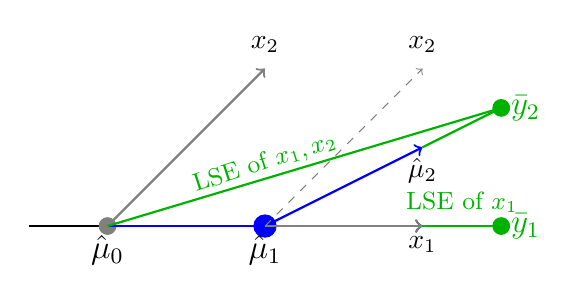
\begin{tikzpicture}
            % First TikZ diagram content
            % Axes
            \draw[->, thick] (-1, 0) -- (4,0) node[below] {$x_1$};

            % Points
            \filldraw[gray] (0, 0) circle (3pt) node[below, black] {\large $\hat{\mu}_0$};
            \filldraw[blue] (2, 0) circle (4pt) node[below, black] {\large $\hat{\mu}_1$};

            % Vectors
            \draw[blue, thick, ->] (0, 0) -- (2, 0);
            \draw[blue, thick, ->] (2, 0) -- (4, 1);
            \node[black] at (4, 0.7) {$\hat{\mu}_2$};

            \draw[gray, thick, ->] (2, 0) -- (4, 0);
            \draw[gray, thick, ->] (0, 0) -- (2, 2);
            \node[black] at (2, 2.3) {$x_2$};

            \draw[gray, dashed, ->] (2, 0) -- (4, 2);
            \node[black] at (4, 2.3) {$x_2$};

            \draw[green!70!black, thick] (0, 0) -- (5, 1.5);
            \draw[green!70!black, thick] (4, 0) -- (5, 0);
            \draw[green!70!black, thick] (4, 1) -- (5, 1.5);

            % Labels
            \filldraw[green!70!black] (5, 1.5) circle (3pt) node[right] {\large $\bar{y}_2$};
            \node[green!70!black, rotate = 18] at (2, 0.8) {\small LSE of $x_1, x_2$};

            \filldraw[green!70!black] (5, 0) circle (3pt) node[right] {\large $\bar{y}_1$};
            \node[green!70!black] at (4.5, 0.3) {\small LSE of $x_1$};
        \end{tikzpicture}
        \caption{Second step in LAR proceduere.}
    \end{minipage}
    \hfill
    \begin{minipage}[t]{0.48\textwidth}
        \centering
        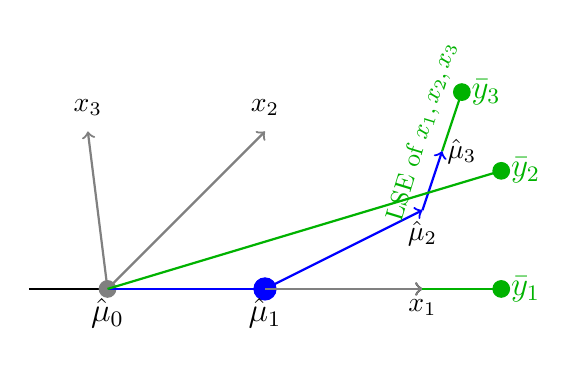
\begin{tikzpicture}
            % Second TikZ diagram content
            % Axes
            \draw[->, thick] (-1, 0) -- (4,0) node[below] {$x_1$};

            % Points
            \filldraw[gray] (0, 0) circle (3pt) node[below, black] {\large $\hat{\mu}_0$};
            \filldraw[blue] (2, 0) circle (4pt) node[below, black] {\large $\hat{\mu}_1$};

            % Vectors
            \draw[blue, thick, ->] (0, 0) -- (2, 0);
            \draw[blue, thick, ->] (2, 0) -- (4, 1);
            \node[black] at (4, 0.7) {$\hat{\mu}_2$};
            \draw[blue, thick, ->] (4, 1) -- (4.25, 1.75);
            \node[black] at (4.5, 1.75) {$\hat{\mu}_3$};

            \draw[gray, thick, ->] (2, 0) -- (4, 0);
            \draw[gray, thick, ->] (0, 0) -- (2, 2);
            \node[black] at (2, 2.3) {$x_2$};

            \draw[gray, thick, ->] (0, 0) -- (-0.25, 2);
            \node[black] at (-0.25, 2.3) {$x_3$};

            \draw[green!70!black, thick] (0, 0) -- (5, 1.5);
            \draw[green!70!black, thick] (4, 0) -- (5, 0);
            \draw[green!70!black, thick] (4.25, 1.75) -- (4.5, 2.5);

            % Labels
            \filldraw[green!70!black] (5, 1.5) circle (3pt) node[right] {\large $\bar{y}_2$};
            \filldraw[green!70!black] (5, 0) circle (3pt) node[right] {\large $\bar{y}_1$};
            \filldraw[green!70!black] (4.5, 2.5) circle (3pt) node[right] {\large $\bar{y}_3$};

            \node[green!70!black, rotate = 73] at (4, 2) {\small LSE of $x_1, x_2, x_3$};
        \end{tikzpicture}
        \caption{Third step in LAR procedure.}
    \end{minipage}
\end{figure}

Figure 1 and Figure 2 shows the step-wise progression, where the blue line is the solution path and the green lines highlight the least squares errors of $x_1, \dots, x_n$ at the $n$th step. Notice that the feature selected at each step is the one with the next least angle, hence the name least angle regression.

\subsection{Properties}

The fused lasso is inherits properties from both the lasso and fusion penalties. As such, it requires features to be standardized with mean 0 and unit variance. The equation \ref{eq:fusedlasso} has been shown to define a convex problem, which ensures at most $N$ features 
 are selected when $p > N$, provided two conditions are met: (1) no columns of the design matrix $X$ are perfectly collinear (linearly dependent), and (2) there is no solution for a set of $N - 1$ linear equations with $N$ variables. 

 One could also see that the degrees of freedom of a fused lasso fit naturally correspond to the number of distinct blocks of nonzero coefficients:

\[\text{df}(\hat{y}) = \#\{\text{non-zero coefficient blocks in }\hat{\beta}\}\]

\noindent since all coefficients within a block share the same value and thus contribute only one degree of freedom. This can be more rigorously stated as 

\[\text{df}(\hat{y}) = p - \#\{\beta_j = 0\} - \#\{\beta_j - \beta_{j - 1} = 0, \beta_j, \beta_{j - 1} \ne 0\}.\]

\noindent The fused lasso still inherits a the negative from lasso penalty where when a group of features are highly correlated, it still tends to select just one arbitrarily from the group.

\section{Simulation}

We attempt to recreate the simulation study presented in Tibshirani et al. (2005). In the original setup, the authors used the first 1000 features from a real protein mass spectrometry dataset and a random subset of 100 patient samples. As this dataset was not made available, we generated features instead by sampling from a standard normal distribution with mean 0 and variance 1. 

To approximate the correlation structure of the original data, we simulated features from a multivariate normal distribution with a Toeplitz covariance matrix. This matrix introduces correlation between features using a parameter \(\rho \in [0, 1]\), where \(\rho = 0\) is the same as a univariate normal distribution and \(\rho = 1\) implies perfect correlation (Gray, 2006). In our simulations, we opted for $\rho = 0.2$. The correlation between features $\beta_i$ and $\beta_j$ is determined by their distance, given by $\Sigma_{ij} = \rho^{|j-i|}$, which results in the matrix structure
\[
\Sigma = 
\begin{bmatrix}
1 & \rho & \rho^2 & \cdots & \rho^{p-1} \\
\rho & 1 & \rho & \cdots & \rho^{p-2} \\
\rho^2 & \rho & 1 & \cdots & \rho^{p-3} \\
\vdots & \vdots & \vdots & \ddots & \vdots \\
\rho^{p-1} & \rho^{p-2} & \rho^{p-3} & \cdots & 1
\end{bmatrix}.
\]

We similarly generated coefficient vectors $\beta$ by choosing between 1 and 10 non-overlapping blocks of non-zero coefficients of length between 1 and 100. The values of the non-zero coefficients were sampled from a standard normal distribution. 

The response values were generated with an adjusted error value to Tibshirani (2005) to better visualize the strengths and weaknesses of both implemented models: lasso and fused lasso.
\[y = X\beta + Z,\]
\[20Z \sim N(0, 1).\]

We split the training and test sets such that that 20\% of the data set was used as a test set and the remaining for training. While we used the \texttt{genlasso} package (Arnold \& Tibshirani, 2016) for fused lasso fits, we instead used the \texttt{glmnet} package (Friedman et al., 2010) to utilize its built-in cross-validation capability and computational efficiency.

The package used for fused lasso has a slightly different penalty equation
\[\frac12 \sum_{j = 1}^{p} (y_j - x_j^T \beta_j)^2 + \lambda \sum_{j = 2}^{p} \left|\beta_j - \beta_{j - 1}\right| + \gamma \cdot \lambda \sum_{j=1}^{p} \left|\beta_j\right|\]

\noindent where $\lambda$ controls the fusion penalty and $\gamma \ge 0$ sets the strength of the lasso penalty relative to the fusion penalty.

For each Monte Carlo simulation, we computed the lasso solution that minimized test error. For fused lasso, we performed a modified grid search over the two penalty parameters, $\lambda$ and $\gamma$. Specifically, we tested values of $\gamma$ from 0.1 to 5 in increments of 0.1. Note, we excluded $\gamma = 0$ since this corresponds to the pure fusion case. For each $\gamma$, we evaluated over the full solution path and selected the combination of $\gamma$ and $\lambda$ which minimized test error. In total, we ran 100 Monte Carlo simulations to evaluate model performance. We used the same metrics, sensitivity and specificity, to assess model performance:

\vspace{0.5cm}

\textbf{Sensitivity} — the proportion of true non-zero coefficients correctly identified
\[\text{Sensitivity} = \frac{\text{True Positives}}{\text{True Positives} + \text{False Negatives}}\]

\textbf{Specificity} — the proportion of true zero coefficients correctly identified
\[\text{Specificity} = \frac{\text{True Negatives}}{\text{True Negatives} + \text{False Positives}}\]

These metrics measured each model's ability to identify true non-zero coefficients while balancing true positives and false positives.

\subsection{Results and Discussion}

Our simulation results reflect the same qualitative trends observed by Tibshirani (2005). As can be seen in Table \ref{tab:simulation_results},

\begin{table}[H]
\centering
    \begin{threeparttable}
        \caption{Results of the simulation study\tnote{\dag}}
        \label{tab:simulation_results}
        \begin{tabular}{lccc}
            \toprule
            \textbf{Method} & \textbf{Test error} & \textbf{Sensitivity} & \textbf{Specificity} \\
            \midrule
            Lasso & 634.7853 (35.5113) & 0.0313 (0.0041) & 0.9764 (0.0276) \\
            Fused Lasso & 514.1339 (25.1243) & 0.3403 (0.0030) & 0.9433 (0.0038) \\
            \bottomrule
            \end{tabular}
        \begin{tablenotes}
            \item[\dag] Standard errors are given in parentheses.
        \end{tablenotes}
    \end{threeparttable}
\end{table}

\noindent the fused lasso has a lower test error compared to lasso and has higher sensitivity, indicating improved detection of non-zero coefficients. There is a tradeoff however, at the cost of lower specificity, causing slightly more false positives. This overall positive tradeoff however lead to a significantly longer computational time.  

Despite these similarities between Tibshirani (2005) and our simulation study, some aspects of the original simulation could not be replicated due lack of access to the original prostate cancer dataset. To approximate the local feature correlation expected in mass spectrometry data, we generated predictors using a Toeplitz correlation structure, as the fused lasso benefits from such natural orderings. However, the synthetic features were not able to produce similar results without some tuning.

In the original study, approximately 300 observations were available, from which a random subset of 100 was selected. In our case however, new $x_{ij}$'s were generated for each simulation run, likely contributing to a higher standard error across all metrics.

Initially, we matched the original simulation's error distribution using $\varepsilon_{sd} = 2.5$. While this reproduced the patterns in sensitivity, specificity and test error were wildly different. To better highlight the model tradeoffs, we increased error standard deviation to $\varepsilon_{sd} = 20$.

\begin{figure}[H]
    \centering
    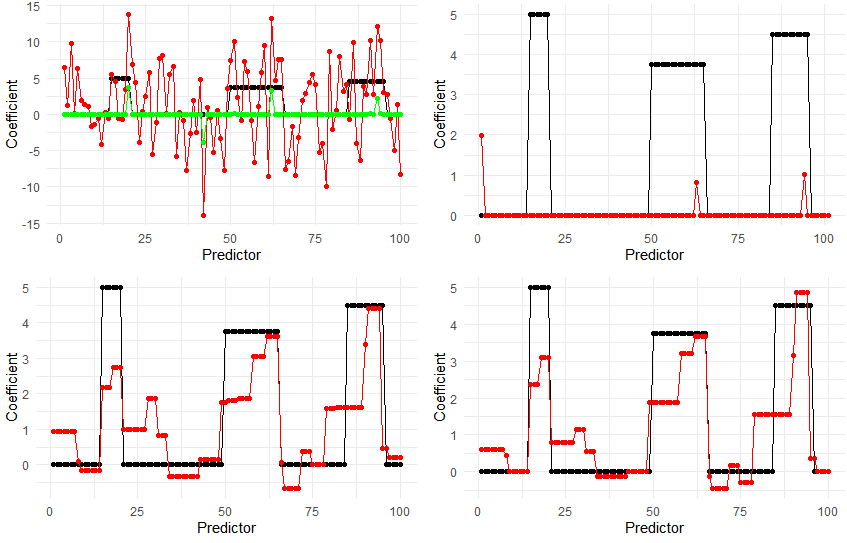
\includegraphics[width = 1\linewidth]{sim-3.png}
    \caption{\footnotesize Simulated example, with $N = 20$ observations and $p = 100$ predictors having coefficients shown by the black lines: (top left) univariate regression coefficients (red) and a soft thresholded version of them (green); (top right) lasso solution (red), (bottom left) fusion estimate (red), using $\gamma = 0$; (bottom right) the fused lasso estimate (red)}
    \label{fig:Tib-3}
\end{figure}

Additionally, we excluded $\gamma = 0$ from our grid of tuning parameters. In early testing, this setting heavily skewed model fitting towards fusion solutions over lasso, rather than balancing both. Even after all modifications though, the average selected $\gamma$ was 0.712. This was likely once again due to the generated feature structure, which closely resembled the simpler example from Section 3 of Tibshirani (2005). An implementation of this setup was also tested, and results are shown in Figure \ref{fig:Tib-3} where it is clear that univariate ($\rho = 0$) feature generation combined with blocky $\beta$ coefficient generation tends to favor fusion. 

Overall, these adjustments helped emphasize the strengths of each model while preserving the variability of the simulated predictors.

\section{Conclusion}

The fused lasso is a powerful extension of the lasso, combining its feature selection ability with an added fusion penalty that accounts for the ordering of features. This makes it well-suited for time series or spatial applications. In our simulation study, the fused lasso demonstrated superior performance to the standard lasso in terms of test error and sensitivity, correctly identifying a larger proportion of non-zero coefficients. However, this came at the cost of lower specificity, giving more false positives, and a significant increase in computational complexity due to the two-dimensional tuning parameter space. Beyond one-dimensional problems, the fused lasso has also been extended to two-dimensional spatial applications, such as image denoising. Future work could apply the fused lasso to real-world ordered datasets to better evaluate its practical utility.

\section{References}

\noindent
\hangindent=1.5em
\hangafter=1
Arnold, T. B., \& Tibshirani, R. J. (2016). Efficient Implementations of the Generalized Lasso Dual Path Algorithm. \textit{Journal of Computational and Graphical Statistics}, 25(1), 1–27. https://doi.org/10.1080/10618600.2015.1008638

\noindent
\hangindent=1.5em
\hangafter=1
Friedman J, Tibshirani R, Hastie T (2010). “Regularization Paths for Generalized Linear Models via Coordinate Descent.” \textit{Journal of Statistical Software}, 33(1), 1–22. doi:10.18637/jss.v033.i01

\noindent
\hangindent=1.5em
\hangafter=1
Gray, R. M. (2006). \textit{Toeplitz and circulant matrices: a review}. Now Publishers, Inc. https://doi.org/10.1561/0100000006

\noindent
\hangindent=1.5em
\hangafter=1
Hastie, T., Taylor, J., Tibshirani, R., \& Walther, G. (2007). Forward stagewise regression and the monotone lasso. \textit{Electronic Journal of Statistics, 1}(none). 

https://doi.org/10.1214/07-EJS004

\noindent
\hangindent=1.5em
\hangafter=1
Land, S., and Friedman, J. (1996). Variable fusion: a new method of adaptive signal regression. \textit{Technical Report}. Department of Statistics, Stanford University, Stanford.

\noindent
\hangindent=1.5em
\hangafter=1
Tibshirani, R. (1996). Regression shrinkage and selection via the lasso. \textit{Journal of the Royal Statistical Society: Series B}, 58(1), 267--288.

\noindent
\hangindent=1.5em
\hangafter=1
Tibshirani, R., Saunders, M., Rosset, S., Zhu, J., \& Knight, K. (2005). Sparsity and smoothness via the fused lasso. \textit{Journal of the Royal Statistical Society. Series B, Statistical Methodology}, 67(1), 91–108. https://doi.org/10.1111/j.1467-9868.2005.00490.x



\end{document}
